\documentclass{article}

\usepackage{nips_2018_author_response}

\usepackage[utf8]{inputenc} % allow utf-8 input
\usepackage[T1]{fontenc}    % use 8-bit T1 fonts
\usepackage{hyperref}       % hyperlinks
\usepackage{url}            % simple URL typesetting
\usepackage{booktabs}       % professional-quality tables
\usepackage{amsfonts}       % blackboard math symbols
\usepackage{nicefrac}       % compact symbols for 1/2, etc.
\usepackage{microtype}      % microtypography
\usepackage{graphicx}


\begin{document}
	

\begin{figure}[!ht]
	\centering
	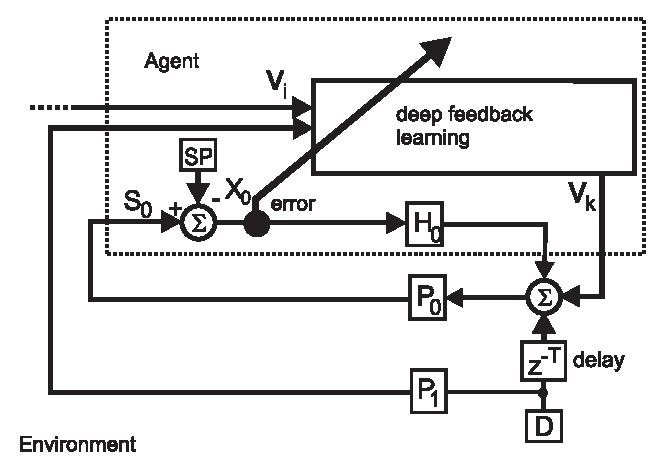
\includegraphics[width=0.55\columnwidth]{closed_loop}
	\caption{
		\label{closed_loop}}
\end{figure}

	
	$H_{0}$ is simply the transfer function of the fixed feedback loop – e.g. if it were a simple thermostat trying to maintain a desired temperature, it would be a threshold function that mapped temperatures onto a binary output. $P_{1}$ is the function that transforms the actions back into sensory inputs $V_{i}$ used for learning. 
	

		
	We have confused several reviewers with the term 'reflex', apologies! In figure 1, we see that there is a fixed feedback loop with setpoint SP; this is what we are calling a ``reflex'', as an analogy with the reflex circuits that are often seen in biology. The reflex for the shooter game is rather artificial, but reflexes are common biological control mechanisms for coping with disturbances. However they have the drawback that they are purely reactive. The contribution here is:
	\begin{itemize}
		\item To show that the reflex can also provide a learning signal for training a deep network, and that network is then learning input control rather than output control - it is learning to keep the reflex silent rather than produce target outputs.
		\item To achieve learning where the errors are defined at the inputs, we develop a learning rule is not gradient-based, but rather where both activity and error signals are propagated forwards in the same weighted fashion. The learning rule is then correlation-based between these two signals.
	\end{itemize}
	
	
		Figure 2B simply visualises this weight change rule, where we correlate the activity $v_{j}$ at neuron $j$ with the error signal $e_{k}$ at neuron $k$. This is identical to backpropagation of course - the key difference lies in the fact that the error is calculated at the inputs, as is the case in closed loop systems. This error can not only be that of a feedback controller, but also for example the TD error of temporal difference learning / reinforcement learning. Any error generated in a closed loop can be used.
		
		
		
	The reason we would expect more behavioural flexibility from this approach is that learning does not explicitly evaluate the network outputs at all. Of course, the inputs do relate to the outputs, but only indirectly, and only via the transfer function $P_{0/1}$ of the environment. So the outputs are less constrained than they would be under Q-learning for example, where the Q value is a direct function of the outputs (and the world state). We should probably say "in principle this leads to greater flexibility", until we show evidence of this. 
	
	
	The goal was to show the feasibility of an algorithm that can function in an arbitrarily deep network. It is true that the actual network used was not particularly deep however. In section 4, we say "let us assume two layers $j$ and $k$", but this is merely to illustrate how the learning in one layer relates to its neighbouring layer.  
	
	For the shooter example, unfortunately some details have been lost during editing. There are 3 output neurons with $tanh$ activation; a negative output means ‘rotate left’, a positive ‘rotate right’. The 3 neurons operate with different gains, to give finer control. The terms $g_{net}$ and $g_{err}$ are the gains for the reflex, and the learned control signal.
	Momentum was 0.5; weights initialiased in a zero-mean uniform distribution, scaled by the number of weights outputting each neuron.
	
Equation 4: The term $\rho$ is the gain of the fixed feedback loop (the reflex), and can be absorbed into $H_{0}$. 
	
	
Equation 5:
\begin{equation}
\Delta w_{ij} = X_0(z) V_i(-z) \nonumber
\end{equation}
is simply a correlation of $X_{0}$ with $V_{i}$, and . The term $(-z)$ appears because correlation involves reversing one of the signals in time. 

	
\end{document}
